\subsection*{alu control}

The ALU control unit is used to tell the ALU what to do with its inputs. It takes the function part of the instruction and the alu\_op as inputs. The alu\_op is decided by the main control unit based on the opcode of the instruction. The ALU control has two outputs; alu\_func, a four-bit bus with operation details for the ALU, and jump\_alu\_result, used to determine whether or not to jump using the jr instruction. The alu control block is represented in figure \ref {fig:alu_control}
\begin{figure}
	\label{fig:alu_control}
	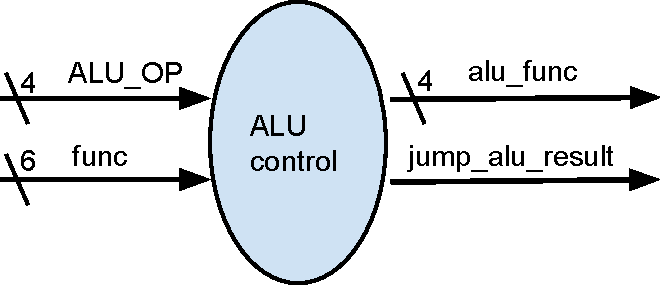
\includegraphics{figures/alu_control}
	\caption{The ALU control block}
\end{figure}

The alu\_input signal consists of four bits, op 0 through 3. Different combinations of high and low bits in this signal will tell the ALU what operation is to be applied to its inputs.  The different results alu\_func can be set to is shown in table \ref{table:alu_control_table}. Note that the order the operands of alu\_func are set up here is for convenience. As long as the operands is set correctly (e.g. op1 <= '1' others => '0' for an add), the order of representation is irrelevant. 

\begin{table}
	\label{table:alu_control_table}
    \begin{tabular}{|l|l|l|l|}
    \hline
    alu\_op           				& \multicolumn {2}{*}{function} 	& alu_input\\(op0, op1, op2, op3) \\ \hline
    \multirow {6}{*}{ALUOP\_FUNC}	& 100000   & add         			& 0100                            \\
                    				& 100010   & subtract  	 			& 0110                            \\
                    				& 100100   & bitwise and 			& 0000                            \\
                    				& 100101   & bitwise or    			& 1000                            \\
                    				& 101010   & set less than 			& 1110                            \\
									& 001000   & jump register 			& 0100                            \\ \hline
    ALUOP\_LOAD_STORE 				& \multicolumn {2}{*}{X}			& 0100                            \\ \hline
    ALUOP\_BRANCH     				& \multicolumn {2}{*}{X} 			& 0110                            \\ \hline
    ALUOP\_LDI        				& \multicolumn {2}{*}{X} 			& 0001                            \\ \hline
    \end{tabular}
\end{table}

The jump register function is controlled from the ALU control unit. It will result in the same input control as add, but the constant being added to the input is always 0. This means that the register address the ALU returns is the same as it gets as input. 

If the operation called is a branch, the input to the ALU is identical to a normal subtraction call. This is because the operation requires two registers to be equal to be able to branch. The easiest way to check if two registers are equal is to subtract one from the other, and if the result is 0, then a line called zero is set high and used as a control signal. 

The load/store operation will also result in an add instruction to the ALU. This is done because to be able to choose what position in the register you should write from or to. 

